\subsection{Evaluation of Diffusion Quality}
\label{sec:eval_vis}
%\todo{better title?}
%
By computing the shift values $t_f$ only for some of the vertices of $M$, and
obtaining them at the other vertices by diffusion we introduce an error.
%
We quantify this error as the normalized absolute difference between a ground
truth and the values at each vertex after the diffusion process.
%
The ground truth is obtained by computing the model parameters $t_f$ for each
vertex of $M$ as described in \cref{sub:fitting}.
%
The diffusion error $e^{V,f}_{\textnormal{diff}}$ for variable $V$ and feature
$f$ is defined as
%
\begin{equation}
	e^{V, f}_{\textnormal{diff}} = \frac{1}{\max(t^V_f)-\min(t^V_f)}
		\Sum{
			\left|
				{t^V_{fi} - t'^{V}_{fi}}
			\right|}{\vm_i \in M}
			\text{ ,}
\end{equation}
%
where $t^V_{fi}$ is the true shift value for variable $V$ and feature $f$ at
vertex $\vm_i$, $t'^{V}_{fi}$ is the corresponding value obtained by
diffusion, and $\max(t^V_f)-\min(t^V_f)$ is the range of true shift values over
all vertices.
%
We computed this error metric for all variables and time steps of
data set \textsc{Hydrogen}, using different seeding densities $q$.
%
We show the results in \cref{fig:diffusion_quality,fig:diffusion_quality_img}.
% An appropriate seeding density $q$ for a desired diffusion quality
% and therefore accuracy of visualization can be automatically determined by
% successively lowering $q$ and computing $e^{V, f}_{\textnormal{diff}}$
% until a satisfactory error level is reached.
% \todo{captain obvious?}

\begin{figure}[t]
	\tikzset{external/export next=false}
	\setlength\figureheight{4.5cm}
	\setlength\figurewidth{0.85\textwidth}
	\centering
	%
\pgfplotstableread[col sep=comma]{figures/hydrogen_TEMP_diff_err.csv}\tempdata
\pgfplotstableread[col sep=comma]{figures/hydrogen_O_diff_err.csv}\odata
\pgfplotstableread[col sep=comma]{figures/hydrogen_OH_diff_err.csv}\ohdata
\pgfplotstableread[col sep=comma]{figures/hydrogen_H2O2_diff_err.csv}\htotdata
\pgfplotstableread{figures/hydrogen_TEMP_diff_err_stat.csv}\tempstat
\pgfplotstableread{figures/hydrogen_O_diff_err_stat.csv}\ostat
\pgfplotstableread{figures/hydrogen_OH_diff_err_stat.csv}\ohstat
\pgfplotstableread{figures/hydrogen_H2O2_diff_err_stat.csv}\htotstat
\pgfplotstableread[col sep=comma]{figures/seeding_densities.csv}\densities

\pgfplotstableset{
	create on use/densities/.style={create col/copy column from table={\densities}{[index] 0}}
}

%\pgfdeclareimage{img1}{figures/diffusion_quality_1.00}
%\pgfdeclareimage{img2}{figures/diffusion_quality_6.70}
%\pgfdeclareimage{img3}{figures/diffusion_quality_36.00}
%\pgfdeclareimage{img4}{figures/diffusion_quality_240.00}
% \definecolor{mycolor1}{HTML}{462390}%
% \definecolor{mycolor2}{HTML}{C30052}%
% \definecolor{mycolor3}{HTML}{D27221}%
% \definecolor{mycolor4}{HTML}{6FBE1E}%

\begin{tikzpicture}

\pgfplotsset{
    small,
	width=\figurewidth,
	height=\figureheight,
	scale only axis,
    every tick/.style={color=black, thin},
	xmode=log,
}

\begin{axis}[%
    axis y line* = left,
    axis x line* = box,
    tick pos = left,
    xmin = 1,
    xmax = 240,
    xminorticks = true,
    %xtick = {1, 4.7, 6.7, 11.5, 16, 23.3, 36, 58, 240},
    xlabel = {$\seedDensQuot$},
    xlabel near ticks,
    xmode = log,
    %
    ymin=0,
    ymax=0.4,
    ylabel={$E^{V, f}_\text{diff}$},
    every axis y label/.style={ at={(rel axis cs:-0.15, 0.5)} },
    %ylabel near ticks,
    ytick = {0, 0.05, 0.1, 0.15},
    yticklabels={
    		 	\textcolor{mycolor1}{T},
    		 	\textcolor{mycolor2}{$\text{H}_2\text{O}_2$},
    		 	\textcolor{mycolor3}{O},
    		 	\textcolor{mycolor4}{OH}
    		 },
    ymajorgrids,
    extra description/.code={
    		\xdef\XMIN{\pgfkeysvalueof{/pgfplots/xmin}}
            \xdef\XMAX{\pgfkeysvalueof{/pgfplots/xmax}}
            \xdef\YMIN{\pgfkeysvalueof{/pgfplots/ymin}}
            \xdef\YMAX{\pgfkeysvalueof{/pgfplots/ymax}}
            }
]

\node[anchor=north west](img1) at (rel axis cs:-0.03,1.021){
	\pgfbox[left,top]{
		\pgfimage[width=1.4cm,interpolate=true]{figures/diffusion_quality_1.00}
	}
};

\node[anchor=north west] at (rel axis cs:-0.01,1){
	\textcolor{white}{\small $\mathbf{q = 1}$}
};

\node[anchor=north west](img2) at (rel axis cs:0.22,1.021){
	\pgfbox[left,top]{
		\pgfimage[width=1.4cm,interpolate=true]{figures/diffusion_quality_6.70}
	}
};

\node[anchor=north west] at (rel axis cs:0.24,1){
	\textcolor{white}{\small $\mathbf{q = 6.7}$}
};

\node[anchor=north west](img3) at (rel axis cs:0.47,1.021){
	\pgfbox[left,top]{
		\pgfimage[width=1.4cm,interpolate=true]{figures/diffusion_quality_36.00}
	}
};

\node[anchor=north west] at (rel axis cs:0.49,1){
	\textcolor{white}{\small $\mathbf{q = 36}$}
};

\node[anchor=north west](img4) at (rel axis cs:0.72,1.021){
	\pgfbox[left,top]{
		\pgfimage[width=1.4cm,interpolate=true]{figures/diffusion_quality_240.00}
	}
};

\node[anchor=north west] at (rel axis cs:0.74,1){
	\textcolor{white}{\small $\mathbf{q = 240}$}
};

% Plots for TEMP

\addplot[
color=mycolor1,
solid,thick,
forget plot,
error bars/.cd,
y dir = minus,
y explicit
]
table[x=densities, y expr = \thisrowno{8} + 0.0, y error index = 9]{\tempstat};
\addplot[
color=mycolor1,
solid,thick,
error bars/.cd,
y dir = plus,
y explicit,
]
table[x=densities, y expr = \thisrowno{8} + 0.0, y error index = 10]{\tempstat};

% \addplot [
% color=mycolor1,
% solid,
% line width=1.0pt
% ]
% table[x=densities,y index = 0]{\tempdata};

% \addplot [
% color=mycolor1,
% solid,
% line width=1.0pt
% ]
% table[x=densities,y index = 1]{\tempdata};

% \addplot [
% color=mycolor1,
% solid,
% line width=1.0pt
% ]
% table[x=densities,y index = 2]{\tempdata};

% \addplot [
% color=mycolor1,
% solid,
% line width=1.0pt
% ]
% table[x=densities,y index = 3]{\tempdata};

% \addplot [
% color=mycolor1,
% solid,
% line width=1.0pt
% ]
% table[x=densities,y index = 4]{\tempdata};

% \addplot [
% color=mycolor1,
% solid,
% line width=1.0pt
% ]
% table[x=densities,y index = 5]{\tempdata};

% \addplot [
% color=mycolor1,
% solid,
% line width=1.0pt
% ]
% table[x=densities,y index = 6]{\tempdata};

% \addplot [
% color=mycolor1,
% solid,
% line width=1.0pt
% ]
% table[x=densities,y index = 7]{\tempdata};

% Plots for H2O2

\addplot[
color=mycolor2,
solid,thick,
forget plot,
error bars/.cd,
y dir = minus,
y explicit
]
table[x=densities, y expr = \thisrowno{8} + 0.05, y error index = 9]{\htotstat};
\addplot[
color=mycolor2,
solid,thick,
error bars/.cd,
y dir = plus,
y explicit,
]
table[x=densities, y expr = \thisrowno{8} + 0.05, y error index = 10]{\htotstat};

% \addplot [
% color=mycolor2,
% solid,
% line width=1.0pt
% ]
% table[x=densities, y expr = \thisrowno{0} + 0.05]{\htotdata};

% \addplot [
% color=mycolor2,
% solid,
% line width=1.0pt
% ]
% table[x=densities, y expr = \thisrowno{1} + 0.05]{\htotdata};

% \addplot [
% color=mycolor2,
% solid,
% line width=1.0pt
% ]
% table[x=densities, y expr = \thisrowno{2} + 0.05]{\htotdata};

% \addplot [
% color=mycolor2,
% solid,
% line width=1.0pt
% ]
% table[x=densities, y expr = \thisrowno{3} + 0.05]{\htotdata};

% \addplot [
% color=mycolor2,
% solid,
% line width=1.0pt
% ]
% table[x=densities, y expr = \thisrowno{4} + 0.05]{\htotdata};

% \addplot [
% color=mycolor2,
% solid,
% line width=1.0pt
% ]
% table[x=densities, y expr = \thisrowno{5} + 0.05]{\htotdata};

% \addplot [
% color=mycolor2,
% solid,
% line width=1.0pt
% ]
% table[x=densities, y expr = \thisrowno{6} + 0.05]{\htotdata};

% \addplot [
% color=mycolor2,
% solid,
% line width=1.0pt
% ]
% table[x=densities, y expr = \thisrowno{7} + 0.05]{\htotdata};

% Plots for O

\addplot[
color=mycolor3,
solid,thick,
forget plot,
error bars/.cd,
y dir = minus,
y explicit
]
table[x=densities, y expr = \thisrowno{8} + 0.1, y error index = 9]{\ostat};
\addplot[
color=mycolor3,
solid,thick,
error bars/.cd,
y dir = plus,
y explicit,
]
table[x=densities, y expr = \thisrowno{8} + 0.1, y error index = 10]{\ostat};

% \addplot [
% color=mycolor3,
% solid,
% line width=1.0pt
% ]
% table[x=densities, y expr = \thisrowno{0} + 0.1]{\odata};

% \addplot [
% color=mycolor3,
% solid,
% line width=1.0pt
% ]
% table[x=densities, y expr = \thisrowno{1} + 0.1]{\odata};

% \addplot [
% color=mycolor3,
% solid,
% line width=1.0pt
% ]
% table[x=densities, y expr = \thisrowno{2} + 0.1]{\odata};

% \addplot [
% color=mycolor3,
% solid,
% line width=1.0pt
% ]
% table[x=densities, y expr = \thisrowno{3} + 0.1]{\odata};

% \addplot [
% color=mycolor3,
% solid,
% line width=1.0pt
% ]
% table[x=densities, y expr = \thisrowno{4} + 0.1]{\odata};

% \addplot [
% color=mycolor3,
% solid,
% line width=1.0pt
% ]
% table[x=densities, y expr = \thisrowno{5} + 0.1]{\odata};

% \addplot [
% color=mycolor3,
% solid,
% line width=1.0pt
% ]
% table[x=densities, y expr = \thisrowno{6} + 0.1]{\odata};

% \addplot [
% color=mycolor3,
% solid,
% line width=1.0pt
% ]
% table[x=densities, y expr = \thisrowno{7} + 0.1]{\odata};

% Plots for OH

\addplot[
color=mycolor4,
solid,thick,
forget plot,
error bars/.cd,
y dir = minus,
y explicit
]
table[x=densities, y expr = \thisrowno{8} + 0.15, y error index = 9]{\ohstat};
\addplot[
color=mycolor4,
solid,thick,
error bars/.cd,
y dir = plus,
y explicit,
]
table[x=densities, y expr = \thisrowno{8} + 0.15, y error index = 10]{\ohstat};

% \addplot [
% color=mycolor4,
% solid,
% line width=1.0pt
% ]
% table[x=densities,y expr = \thisrowno{0} + 0.15]{\ohdata};

% \addplot [
% color=mycolor4,
% solid,
% line width=1.0pt
% ]
% table[x=densities,y expr = \thisrowno{1} + 0.15]{\ohdata};

% \addplot [
% color=mycolor4,
% solid,
% line width=1.0pt
% ]
% table[x=densities,y expr = \thisrowno{1} + 0.15]{\ohdata};

% \addplot [
% color=mycolor4,
% solid,
% line width=1.0pt
% ]
% table[x=densities,y expr = \thisrowno{1} + 0.15]{\ohdata};

% \addplot [
% color=mycolor4,
% solid,
% line width=1.0pt
% ]
% table[x=densities,y expr = \thisrowno{1} + 0.15]{\ohdata};

% \addplot [
% color=mycolor4,
% solid,
% line width=1.0pt
% ]
% table[x=densities,y expr = \thisrowno{1} + 0.15]{\ohdata};

% \addplot [
% color=mycolor4,
% solid,
% line width=1.0pt
% ]
% table[x=densities,y expr = \thisrowno{1} + 0.15]{\ohdata};

% \addplot [
% color=mycolor4,
% solid,
% line width=1.0pt
% ]
% table[x=densities,y expr = \thisrowno{1} + 0.15]{\ohdata};
\end{axis}

\begin{axis}[% --- CF
        xmin=\XMIN,
        xmax=\XMAX,
        ymin=\YMIN,
        ymax=\YMAX,
        ticklabel pos=right,        
		axis y line* = right,
		axis x line = none,
		ytick = {0, 0.05, 0.1, 0.15, 0.2, 0.25, 0.3},
		yticklabel style = {%/pgf/number format/precision=3,
							/pgf/number format/fixed}
    ]
\end{axis}

\end{tikzpicture}
	\vspace*{-2mm}
	\caption{
		Diffusion error (median, max and min) for selected variables of data set
		\textsc{Hydrogen}. Qualitative results for the values indicated by vertical
		lines are shown in \cref{fig:diffusion_quality_img}.}
	\label{fig:diffusion_quality}
\end{figure}

\begin{figure}[t]
	\setlength\figurewidth{\textwidth}
	\centering
	\begin{tikzpicture}[
    font=\small,
    node distance=0.25cm,
    every node/.style={inner sep=0pt, outer sep=0pt}
]
    \node (img1) {
        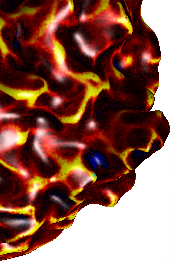
\includegraphics[width=0.25\figurewidth-0.25cm*3/4]{figures/diffusion_quality_1_00.png}
    };
    \node[anchor=north, below=of img1] {$q=1$};

    \node[right=of img1] (img2) {
        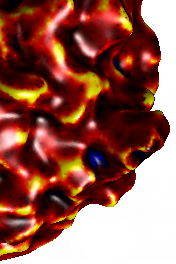
\includegraphics[width=0.25\figurewidth-0.25cm*3/4]{figures/diffusion_quality_6_70.png}
    };
    \node[anchor=north, below=of img2] {$q=6.7$};

    \node[right=of img2] (img3) {
        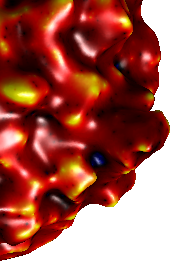
\includegraphics[width=0.25\figurewidth-0.25cm*3/4]{figures/diffusion_quality_36_00.png}
    };
    \node[anchor=north, below=of img3] {$q=36$};

    \node[right=of img3] (img4) {
        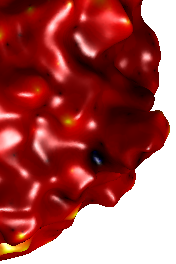
\includegraphics[width=0.25\figurewidth-0.25cm*3/4]{figures/diffusion_quality_240_00.png}
    };
    \node[anchor=north, below=of img4] {$q=240$};
\end{tikzpicture}
	% \vspace*{-5mm}
	\caption{Visual comparison of diffusion results for different seeding
	densities $q$.}
	\label{fig:diffusion_quality_img}
\end{figure}
